\documentclass[12pt,a4paper]{article}
\usepackage[italian]{babel}
\usepackage[T1]{fontenc}
\usepackage[latin1]{inputenc}
\usepackage{graphicx}
\usepackage{amsmath}
\usepackage{subfig}
\date{}
\begin{document}
\title{Strutture Aeronautiche\\ Esercitazione 2 \\ Prof.re Franco Mastroddi}
\author{Matteo Hakimi 1455230}
\maketitle
\begin{figure}[htbp]
\centering

\includegraphics[width=100mm]{Immagini/sapienzalogo}
\end{figure}
\newpage
\tableofcontents
\newpage
\section{Introduzione}
Si vogliono calcolare i primi 10 modi propridi una struttura costituita da un cassone alare incastrato da un lato ,in lega metallica
leggera (alluminio E=68GPa  $\nu =0.3$  $\rho=2650\frac{Kg}{m^3}$ ) di lunghezza longitudinale pari a L=4m , cross section rettangolare di dimensioni 0.6mx0.1m
costituita da 4 pannelli di spessore t=0.003m , e da 4 irriggidimenti ( longheroni) posti ai vertici della sezione trasversale, che percorrono la struttura nella direzione longitudinale, di sezione pari a $ A=0.0025{m^2} $  , confrontando le prime tre frequenze associate ai modi flessionali a quelle ottenute per via analitica.\\
Sostituendo poi l'alluminio con una lega di acciaio si sono calcolati nuovamente le frequenze proprie di vibrazione.
Inoltre si \'e calcolata il termine $H_{ij}(\omega)$ della matrice di risposta in frequenza, prima in assenza di smorzamento e poi ponendo il coefficiente di smorzamento $\zeta=0.03$, nel caso in cui: i sia il grado di libert\'a dello spostamento verticale (T3) del nodo 13 e j il grado di libert\'a dello spostamento anch'esso verticale (T3) del nodo 8, e nel caso in cui: i sia il grado di libert\'a dello spostamento verticale (T3) del nodo 13 e j il grado di libert\'a dello spostamento longitudinale (T1) del nodo 8.
Infine si sono cambiate le condizioni al contorno del cassone alle due estremit�,cio� ponendo in esse delle cerniere con asse di rotazione parallelo all'asse x, e si sono nuovamente calcolati modi e frequenze proprie confrontandoli con quelli offerti dalla teoria analitica.\\
\begin{figure}[htbp]
	\centering
	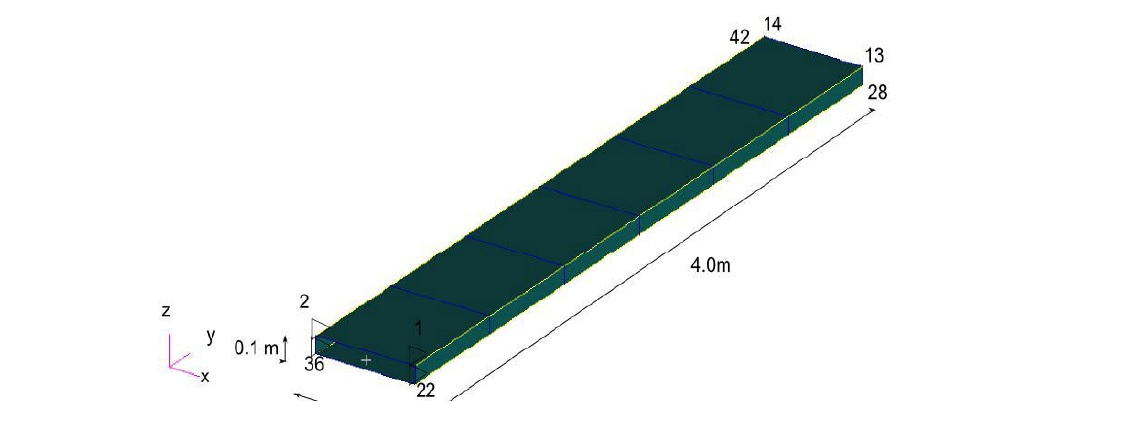
\includegraphics[width=150mm]{Immagini/Cassone}
	\caption{Cassone Alare}
\end{figure}
\section{Calcolo frequenze naturali e modi di vibrazione}
In questo parte verranno calcolate le frequenze proprie nonch\'e i modi di vibrazione, della struttura riportata in figura 1.1, attraverso l'uso del solutore FEM SOL 103,normalizzando quest'ultimi rispetto allo spostamento massimo (usando il comando MAX).\\
Per poter classificare le varie forme modali sono stati selezionati i gradi di libert\'a dei nodi lungo un longherone,data la simmetria della struttura.\\
Usando poi uno script, realizzato con MatLab, \'e stato possibile dare una rappresentazione grafica di tali autovettori normalizzati (nei nodi lungo l'estensione longitudinale),  in modo di visualizzare al meglio la deformata modale.\\
Data la simmetria della struttura, ci aspettiamo dei modi flessionali e torsionali puri, cio\'e totalmente disaccoppiati;tuttavia questo non si \'e visto nei modi calcolati col solutore FEM (si vedano le tabelle), il motivo \'e dovuto sostanzialmente a errori numerici commessi nel processo di soluzione.
\newpage
\subsection{Modo1}
Il primo modo di vibrazione \'e un modo flessionale attorno a x di pulsazione $\omega_{1}=53,11 [rad/s]$.\\
\\
\begin{center}
\begin{tabular}{lllllll}
\hline
\multicolumn{1}{c}{Point}& T1& T2&T3&R1&R2&R3\\
\hline
    1 &        0 &        0 &        0&        0 &       0&         0\\
    3&    0.0010&   -0.0062&    0.0489 &   0.1299&    0.0203&   -0.0014\\
    5&    0.0005&   -0.0110&    0.1707&    0.2239&    0.0091&    0.0018\\
    7&    0.0004&   -0.0142&    0.3448&    0.2870&    0.0071&   -0.0008\\
    9&    0.0002&   -0.0160&    0.5513&    0.3229&    0.0032&    0.0009\\
   11&    0.0001&   -0.0168&    0.7736&    0.3372&    0.0011&   -0.0004\\
   13&    0.0000&   -0.0169&    1.0000&    0.3392&    0.0001&    0.0004\\
\hline
\end{tabular}\\
\end{center}
\begin{figure}[htbp]
\centering
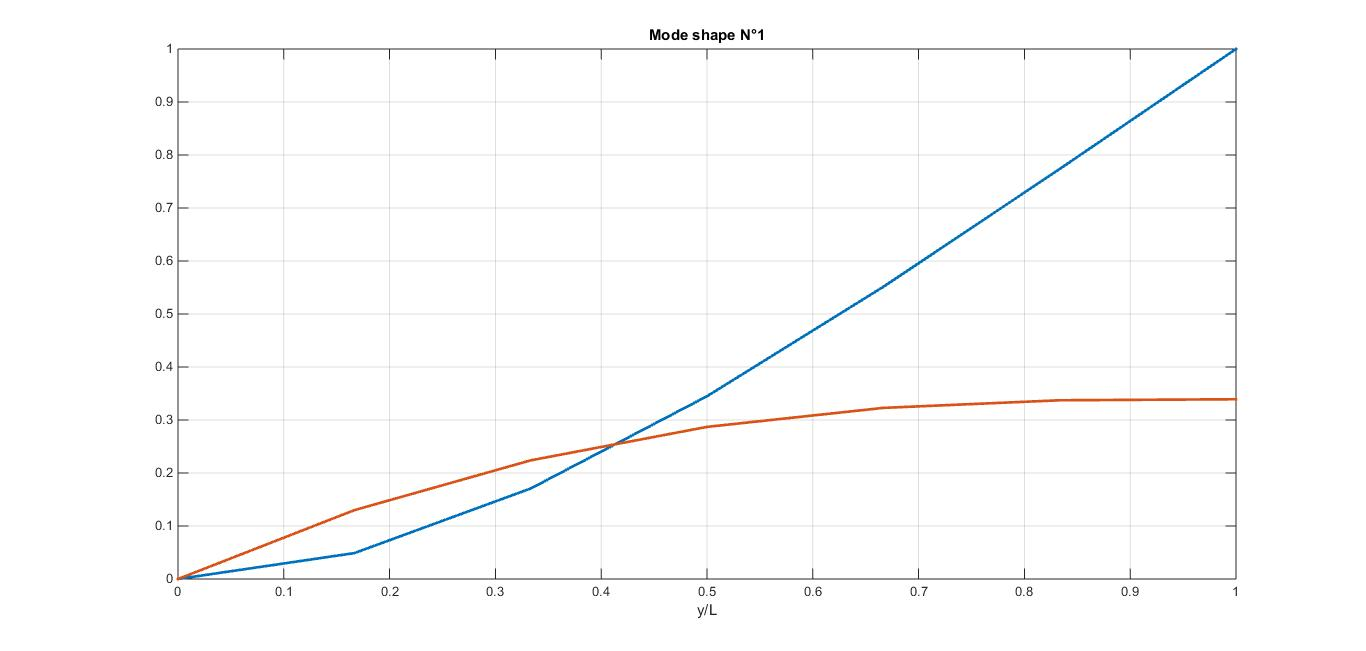
\includegraphics[width=150mm]{Immagini/modo1}
\caption{Modo 1 flessionale attorno a x}
\end{figure}
\newpage
\subsection{Modo2}
Il secondo modo di vibrazione \'e un modo torsionale attorno a y di pulsazione $\omega_{2}=172,18 [rad/s]$.\\
\\
\begin{center}
\begin{tabular}{lllllll}
\hline
\multicolumn{1}{c}{Point}& T1& T2&T3&R1&R2&R3\\
\hline
  1 &   0.0000 &   0.0000 &   0.0000 &   0.0000 &   0.0000 &   0.0000 \\  
  3 &   0.0088 &   0.0109 &  -0.1275 &  -0.3363 &   0.1041 &  -0.0123 \\  
  5 &   0.0033 &   0.0131 &  -0.3385 &  -0.3016 &   0.2507 &   0.0247 \\  
  7 &  -0.0005 &   0.0086 &  -0.5240 &  -0.2308 &   0.4006 &  -0.0086 \\  
  9 &   0.0085 &   0.0003 &  -0.6090 &  -0.0252 &   0.6278 &  -0.0158 \\  
 11 &   0.0339 &  -0.0077 &  -0.5679 &   0.1561 &   0.9207 &  -0.0602 \\  
 13 &   0.0710 &  -0.0111 &  -0.4337 &   0.2329 &   1.0000 &  -0.0414 \\  
\hline
\end{tabular}\\
\end{center}
\begin{figure}[htbp]
\centering
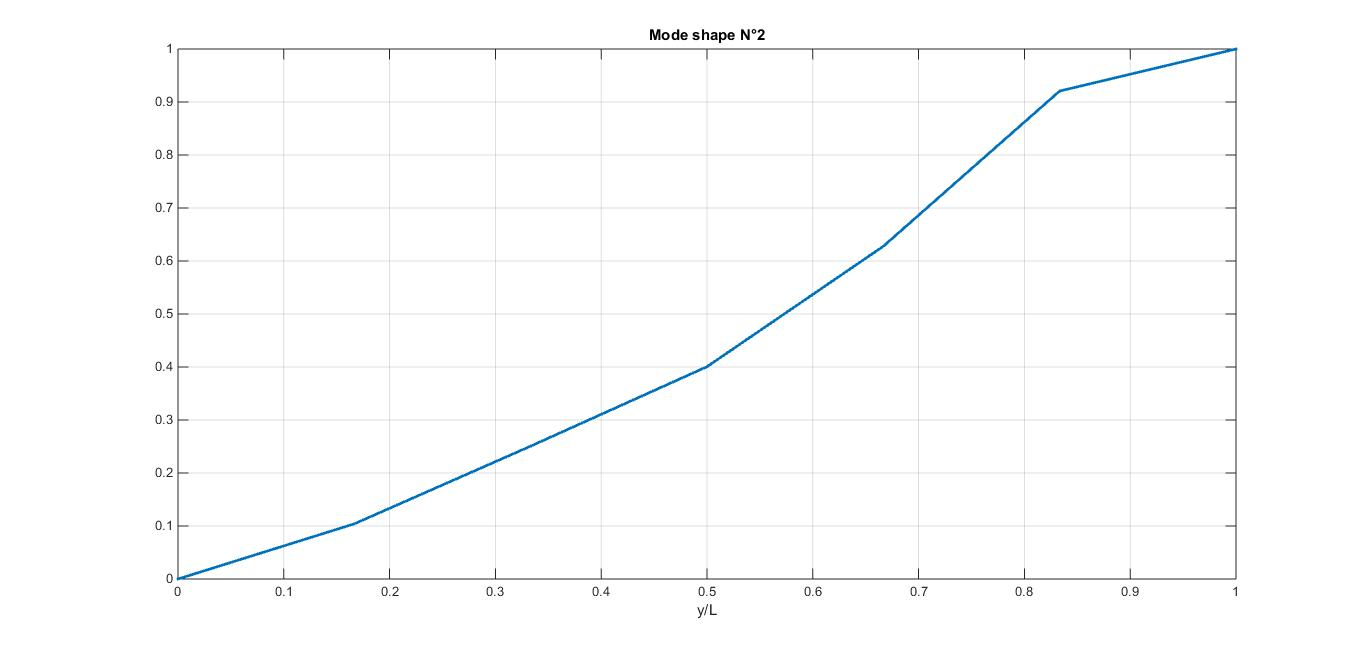
\includegraphics[width=150mm]{Immagini/modo2}
\caption{Modo 2 torsionale attorno a y}
\end{figure}
\newpage
\subsection{Modo3}
Il terzo modo di vibrazione \'e un modo flessionale attorno a z di pulsazione $\omega_{3}=269,54 [rad/s]$.\\
\\
\begin{center}
\begin{tabular}{lllllll}
\hline
\multicolumn{1}{c}{Point}& T1& T2&T3&R1&R2&R3\\
\hline
    1&         0&       0&         0&         0&         0&         0\\
    3 &   0.0701&   -0.0334&    0.0009&    0.0012&   -0.0030&   -0.1329\\
    5& 0.2041&   -0.0584&    0.0004&   -0.0016&   -0.0013&   -0.2148\\
    7&    0.3818&   -0.0752&    0.0003&    0.0007&   -0.0010&   -0.2684\\
    9&   0.5842&   -0.0849&    0.0001&   -0.0008&   -0.0004&   -0.2966\\
   11&    0.7944&   -0.0890&    0.0000&    0.0003&   -0.0001&   -0.3045\\
   13&    1.0000&   -0.0900&    0.0000&   -0.0004&    0.0000&   -0.3042\\
\hline
\end{tabular}\\
\end{center}
\begin{figure}[htbp]
\centering
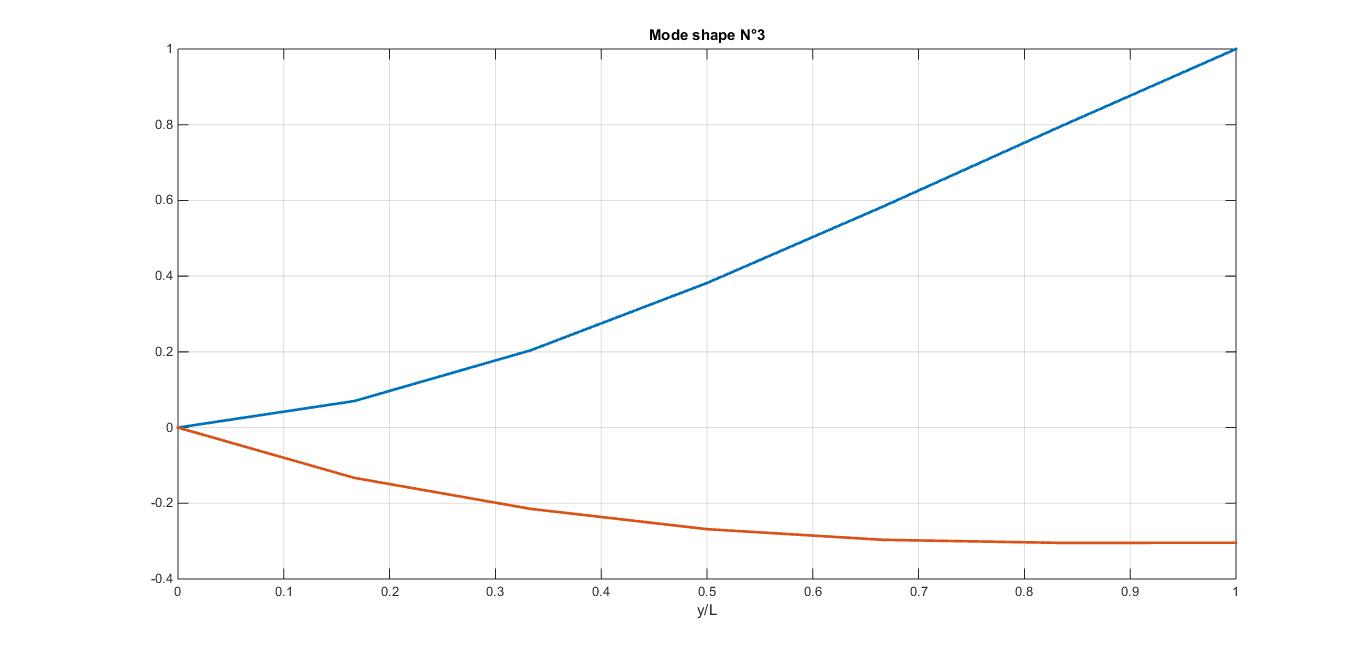
\includegraphics[width=150mm]{Immagini/modo3}
\caption{Modo 3 flessionale attorno a z}
\end{figure}
\newpage
\subsection{Modo4}
Il quarto modo di vibrazione \'e un modo flessionale attorno a x di pulsazione $\omega_{4}=296,63 [rad/s]$.\\
\\
\begin{center}
\begin{tabular}{lllllll}
\hline
\multicolumn{1}{c}{Point}& T1& T2&T3&R1&R2&R3\\
\hline
     1 &   0.0000 &   0.0000 &   0.0000 &   0.0000 &   0.0000 &   0.0000 \\  
  3 &  -0.0021 &   0.0189 &  -0.2460 &  -0.4566 &  -0.0419 &   0.0007 \\  
  5 &   0.0023 &   0.0141 &  -0.5631 &  -0.3283 &   0.0470 &  -0.0087 \\  
  7 &   0.0032 &  -0.0065 &  -0.6582 &   0.1210 &   0.0639 &   0.0034 \\  
  9 &   0.0028 &  -0.0299 &  -0.3980 &   0.6232 &   0.0568 &  -0.0006 \\  
 11 &   0.0012 &  -0.0452 &   0.1576 &   0.9367 &   0.0245 &   0.0041 \\  
 13 &   0.0003 &  -0.0497 &   0.8307 &   1.0000 &   0.0049 &  -0.0010 \\  
\hline
\end{tabular}\\
\end{center}
\begin{figure}[htbp]
\centering
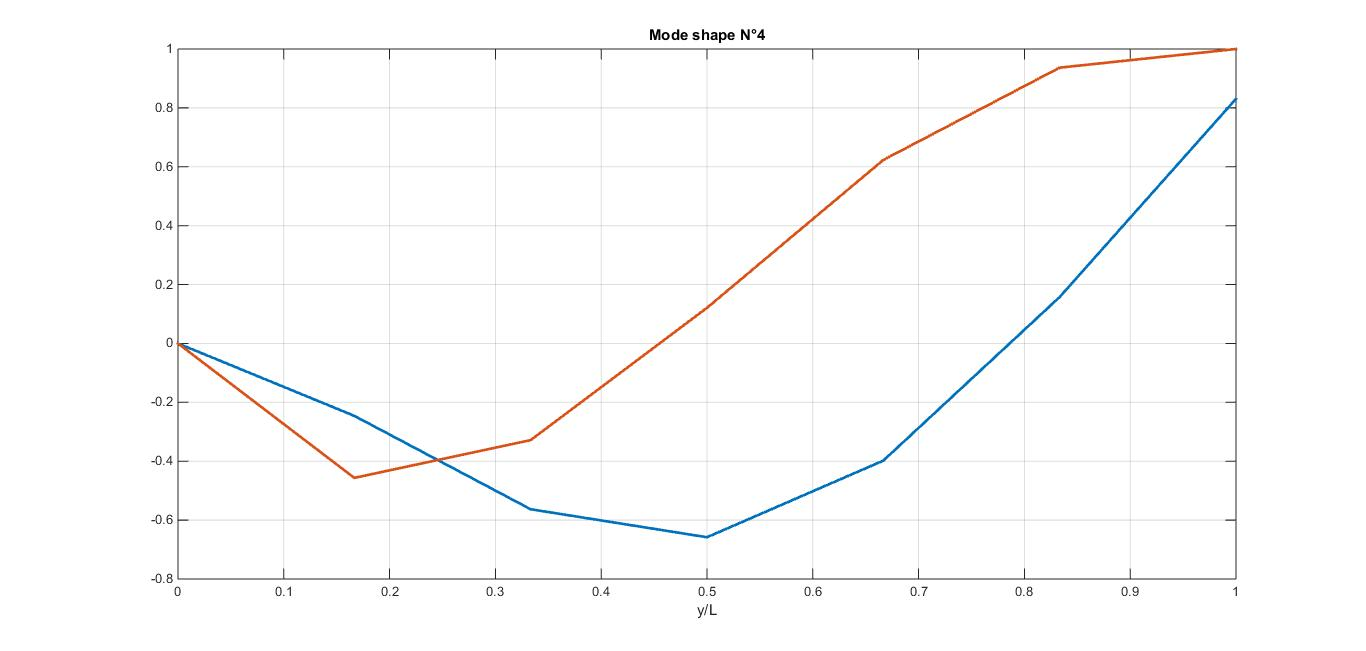
\includegraphics[width=150mm]{Immagini/modo4}
\caption{Modo 4 flessionale attorno a x}
\end{figure}
\newpage
\subsection{Modo5}
Il quinto modo di vibrazione \'e un modo torsionale attorno a y di pulsazione $\omega_{5}=380,44 [rad/s]$.\\
\\
\begin{center}
\begin{tabular}{lllllll}
\hline
\multicolumn{1}{c}{Point}& T1& T2&T3&R1&R2&R3\\
\hline
   1 &   0.0000 &   0.0000 &   0.0000 &   0.0000 &   0.0000 &   0.0000 \\  
  3 &   0.0181 &  -0.0051 &   0.0514 &   0.1391 &   0.2893 &  -0.0444 \\  
  5 &   0.0395 &  -0.0031 &   0.1160 &   0.0569 &   0.5179 &  -0.0210 \\  
  7 &   0.0524 &   0.0025 &   0.1130 &  -0.0674 &   0.7060 &  -0.0142 \\  
  9 &   0.0536 &   0.0074 &   0.0235 &  -0.1926 &   0.8256 &   0.0122 \\  
 11 &   0.0472 &   0.0088 &  -0.1106 &  -0.2004 &   0.8844 &   0.0062 \\  
 13 &   0.0385 &   0.0086 &  -0.2354 &  -0.1708 &   1.0000 &   0.0249 \\  
\hline
\end{tabular}\\
\end{center}
\begin{figure}[htbp]
\centering
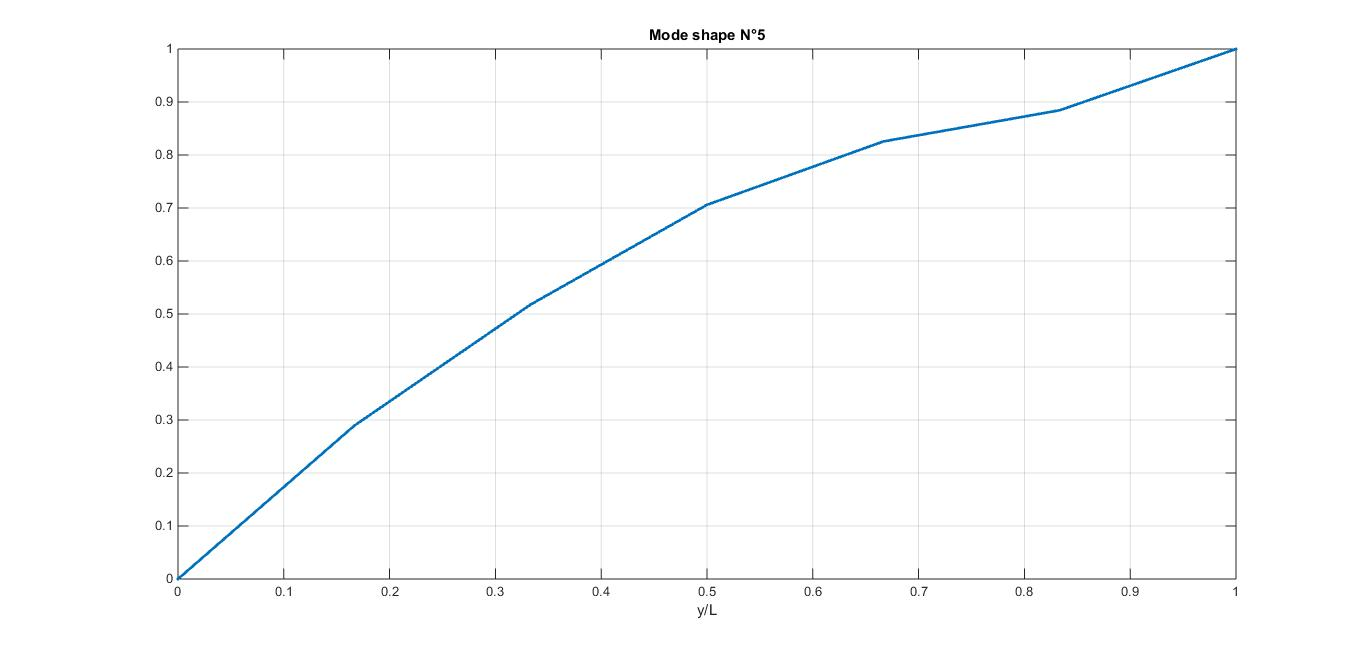
\includegraphics[width=150mm]{Immagini/modo5}
\caption{Modo 5 torsionale attorno a y}
\end{figure}
\newpage
\subsection{Modo6}
Il sesto modo di vibrazione \'e un modo torsionale attorno a y di pulsazione $\omega_{6}=673,54 [rad/s]$.\\
\\
\begin{center}
\begin{tabular}{lllllll}
\hline
\multicolumn{1}{c}{Point}& T1& T2&T3&R1&R2&R3\\
\hline
   1 &   0.0000 &   0.0000 &   0.0000 &   0.0000 &   0.0000 &   0.0000 \\  
  3 &   0.0066 &   0.0047 &  -0.1245 &  -0.2855 &   0.2873 &  -0.0115 \\  
  5 &   0.0177 &  -0.0049 &  -0.1568 &   0.1642 &   0.5714 &  -0.0247 \\  
  7 &   0.0439 &  -0.0109 &  -0.0104 &   0.2776 &   0.7144 &  -0.0483 \\  
  9 &   0.0649 &  -0.0029 &   0.1283 &   0.1108 &   0.7651 &  -0.0147 \\  
 11 &   0.0587 &   0.0106 &   0.0634 &  -0.2956 &   0.7960 &   0.0353 \\  
 13 &   0.0271 &   0.0167 &  -0.1615 &  -0.3548 &   1.0000 &   0.0557 \\  
\hline
\end{tabular}\\
\end{center}
\begin{figure}[htbp]
\centering
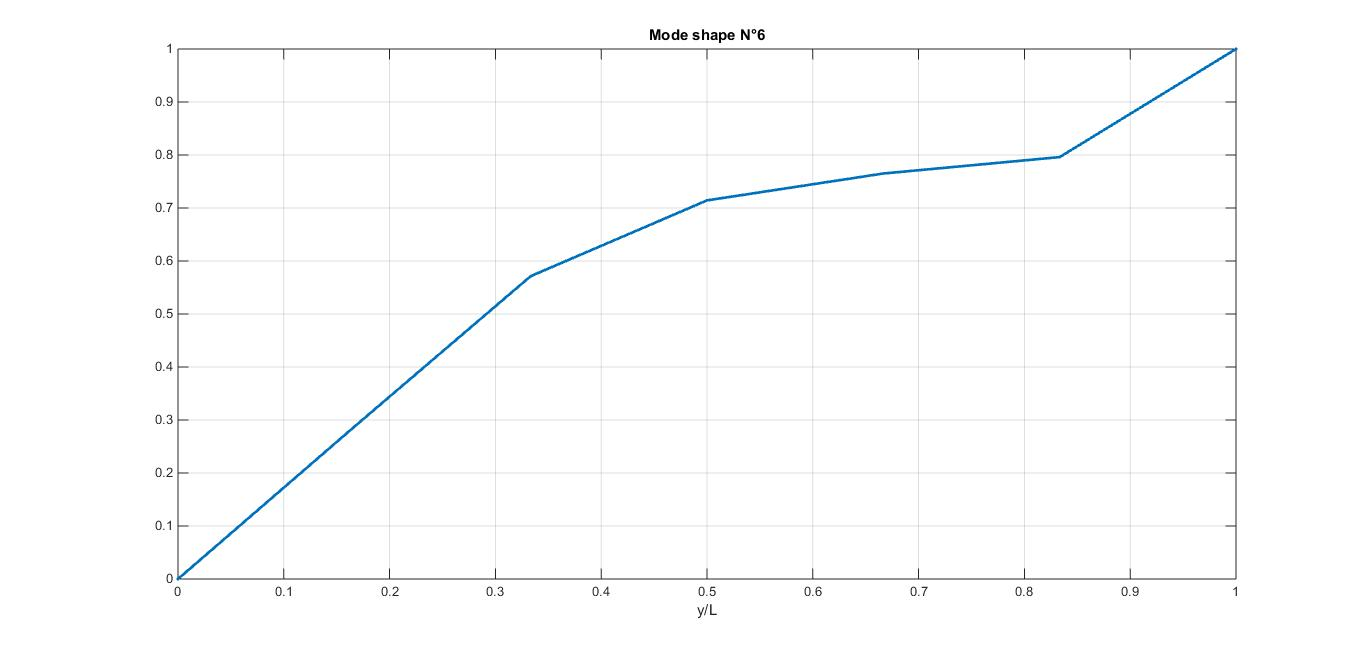
\includegraphics[width=150mm]{Immagini/modo6}
\caption{Modo 6 torsionale attorno a y}
\end{figure}
\newpage
\subsection{Modo7}
Il settimo modo di vibrazione \'e un modo flessionale attorno a x di pulsazione $\omega_{7}=719,66 [rad/s]$.\\
\\
\begin{center}
\begin{tabular}{lllllll}
\hline
\multicolumn{1}{c}{Point}& T1& T2&T3&R1&R2&R3\\
\hline
  1 &   0.0000 &   0.0000 &   0.0000 &   0.0000 &   0.0000 &   0.0000 \\  
  3 &  -0.0001 &  -0.0136 &   0.3778 &   0.4139 &  -0.0027 &   0.0046 \\  
  5 &  -0.0046 &   0.0131 &   0.4599 &  -0.2993 &  -0.0928 &   0.0033 \\  
  7 &   0.0006 &   0.0291 &   0.0036 &  -0.7075 &   0.0124 &  -0.0146 \\  
  9 &   0.0052 &   0.0056 &  -0.4049 &  -0.1574 &   0.1045 &   0.0006 \\  
 11 &   0.0040 &  -0.0324 &  -0.1799 &   0.7230 &   0.0799 &   0.0029 \\  
 13 &   0.0012 &  -0.0490 &   0.5083 &   1.0000 &   0.0225 &   0.0047 \\  
\hline
\end{tabular}\\
\end{center}
\begin{figure}[htbp]
\centering
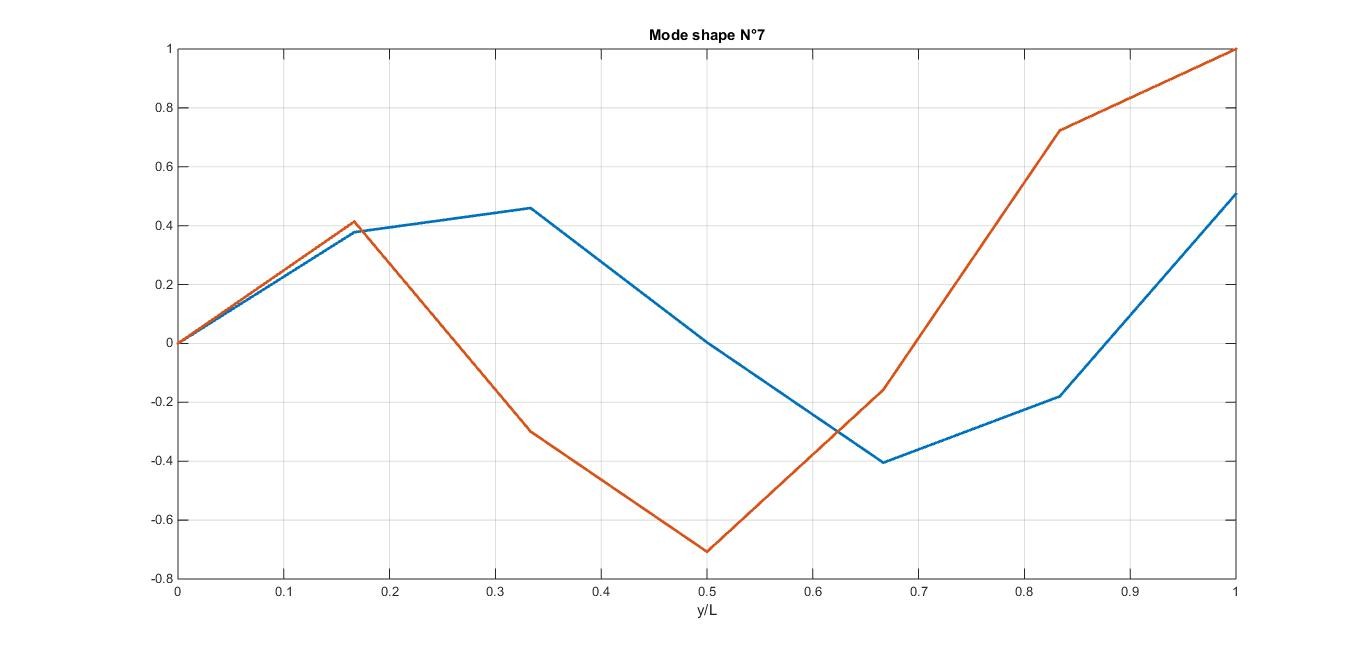
\includegraphics[width=150mm]{Immagini/modo7}
\caption{Modo 7 flessionale attorno a x}
\end{figure}
\newpage
\subsection{Modo8}
l' ottavo modo di vibrazione \'e un modo torsionale attorno a y di pulsazione $\omega_{8}=1118,73 [rad/s]$.\\
\\
\begin{center}
\begin{tabular}{lllllll}
\hline
\multicolumn{1}{c}{Point}& T1& T2&T3&R1&R2&R3\\
\hline
  1 &   0.0000 &   0.0000 &   0.0000 &   0.0000 &   0.0000 &   0.0000 \\  
  3 &   0.0280 &  -0.0026 &   0.1342 &   0.2540 &   0.1830 &  -0.0614 \\  
  5 &   0.0417 &   0.0085 &   0.0346 &  -0.4666 &   0.5940 &   0.0131 \\  
  7 &   0.0427 &   0.0011 &  -0.1356 &  -0.0312 &   1.0000 &  -0.0086 \\  
  9 &   0.0530 &  -0.0087 &  -0.0111 &   0.3959 &   0.8467 &  -0.0271 \\  
 11 &   0.0501 &   0.0030 &   0.1165 &  -0.0804 &   0.5172 &   0.0430 \\  
 13 &   0.0121 &   0.0144 &  -0.0631 &  -0.3816 &   0.6525 &   0.0550 \\  
\hline
\end{tabular}\\
\end{center}
\begin{figure}[htbp]
\centering
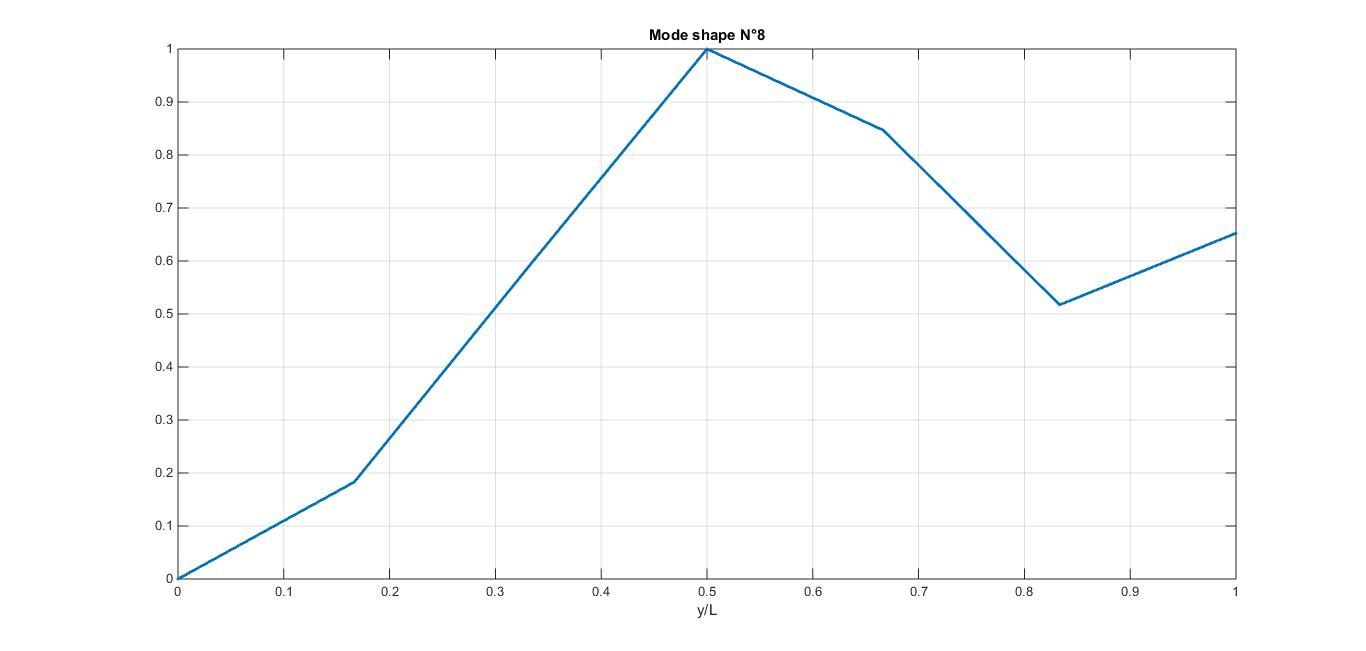
\includegraphics[width=150mm]{Immagini/modo8}
\caption{Modo 8 torsionale attorno a y}
\end{figure}
\newpage
\subsection{Modo9}
Il nono modo di vibrazione \'e un modo flessionale attorno a z di pulsazione $\omega_{9}=1134,95 [rad/s]$.\\
\\
\begin{center}
\begin{tabular}{lllllll}
\hline
\multicolumn{1}{c}{Point}& T1& T2&T3&R1&R2&R3\\
\hline
  1 &   0.0000 &   0.0000 &   0.0000 &   0.0000 &   0.0000 &   0.0000 \\  
  3 &   0.4580 &  -0.0481 &   0.0006 &  -0.0007 &  -0.0021 &  -0.3937 \\  
  5 &   0.8150 &  -0.0034 &  -0.0020 &  -0.0045 &   0.0076 &  -0.1476 \\  
  7 &   0.8260 &   0.0954 &  -0.0024 &   0.0019 &   0.0091 &   0.3047 \\  
  9 &   0.4259 &   0.1965 &  -0.0020 &   0.0001 &   0.0073 &   0.7353 \\  
 11 &  -0.2543 &   0.2599 &  -0.0009 &   0.0025 &   0.0030 &   0.9587 \\  
 13&  -0.9679 &   0.2788 &  -0.0001 &  -0.0002 &   0.0005 &   1.0000 \\  
\hline
\end{tabular}\\
\end{center}
\begin{figure}[htbp]
\centering
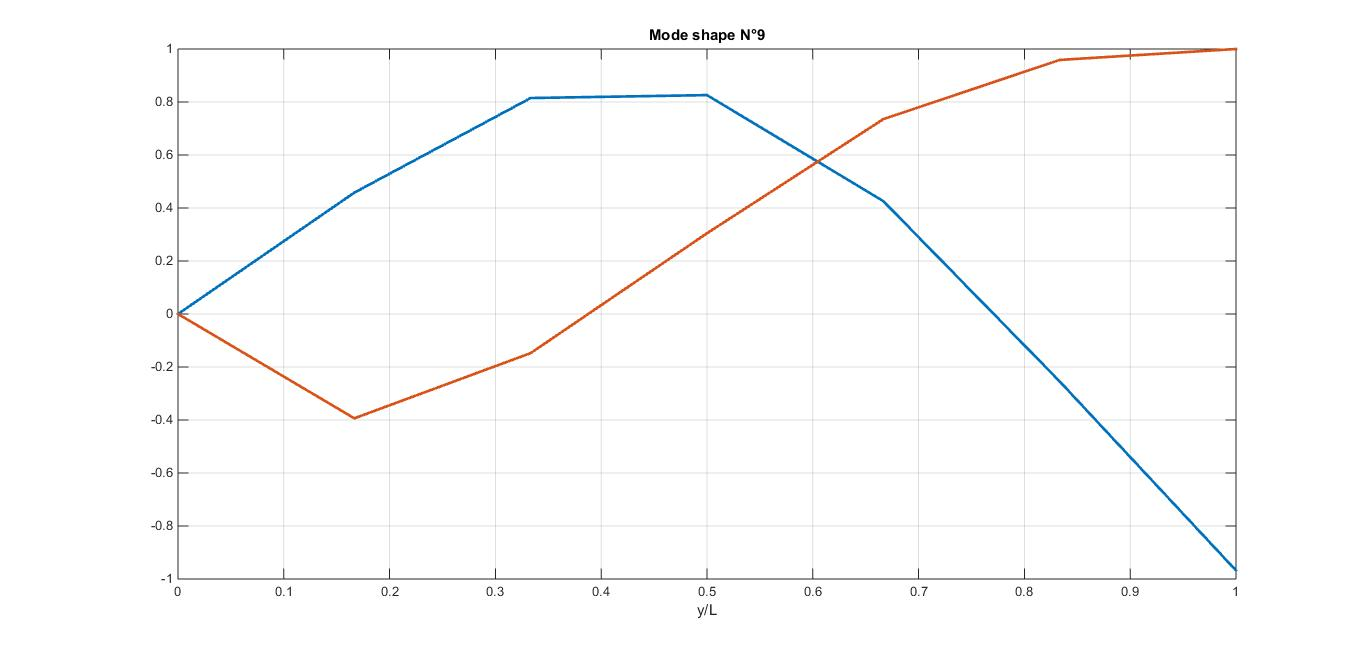
\includegraphics[width=150mm]{Immagini/modo9}
\caption{Modo 9 flessionale attorno a z}
\end{figure}
\newpage
\subsection{Modo10}
Il settimo modo di vibrazione \'e un modo flessionale attorno a x di pulsazione $\omega_{10}=1177,85 [rad/s]$.\\
\\
\begin{center}
\begin{tabular}{lllllll}
\hline
\multicolumn{1}{c}{Point}& T1& T2&T3&R1&R2&R3\\
\hline
 1 &   0.0000 &   0.0000 &   0.0000 &   0.0000 &   0.0000 &   0.0000 \\  
  3 &   0.0027 &  -0.0006 &  -0.4423 &  -0.0959 &   0.0543 &  -0.0073 \\  
  5 &   0.0008 &  -0.0273 &  -0.0489 &   0.7405 &   0.0165 &   0.0146 \\  
  7 &  -0.0060 &   0.0004 &   0.4100 &  -0.0244 &  -0.1217 &   0.0002 \\  
  9 &   0.0017 &   0.0229 &  -0.0716 &  -0.6657 &   0.0338 &  -0.0178 \\  
 11 &   0.0062 &  -0.0158 &  -0.3392 &   0.3535 &   0.1250 &   0.0036 \\  
 13 &   0.0032 &  -0.0478 &   0.3657 &   1.0000 &   0.0592 &   0.0048 \\  
\hline
\end{tabular}\\
\end{center}
\begin{figure}[htbp]
\centering
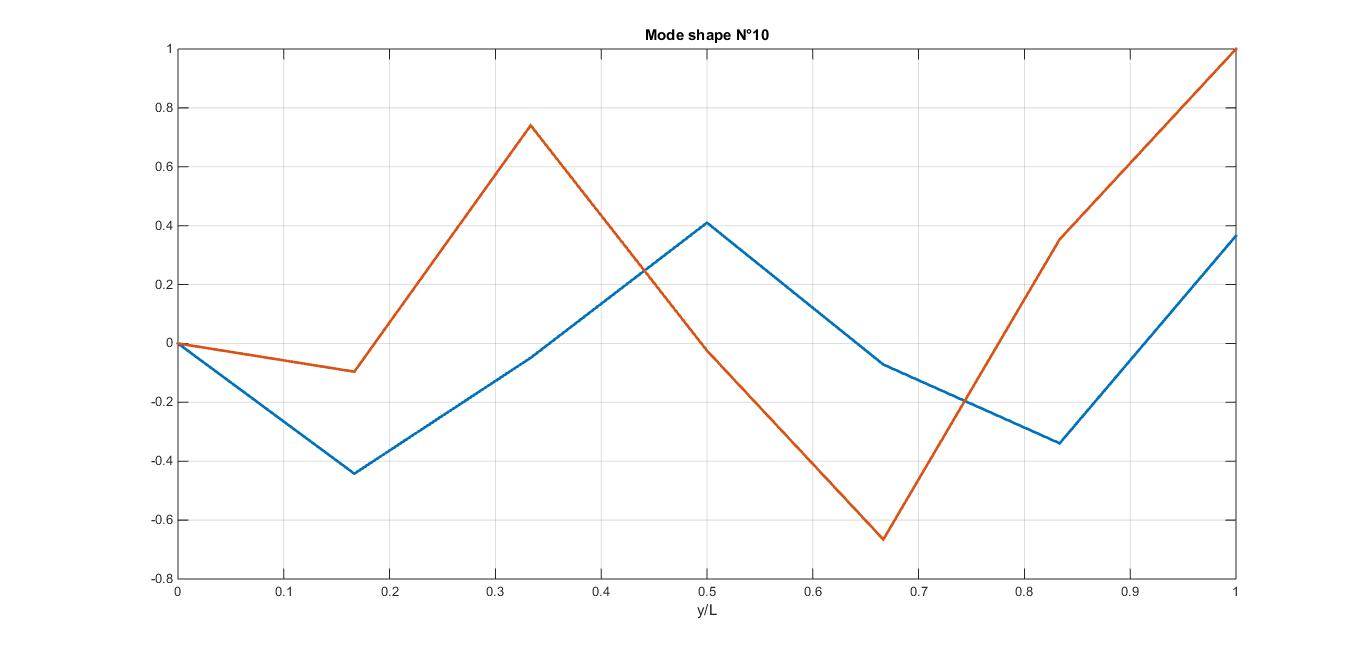
\includegraphics[width=150mm]{Immagini/modo10}
\caption{Modo 10 flessionale attorno a x}
\end{figure}
\newpage
\section{Calcolo frequenze proprie caso acciaio }
Nel caso si avesse una lega in acciaio cambierebbero le matrici di massa e di rigidezza e si prevede che gli autovalori varierebbero secondo questa legge:
\begin{equation}
\lambda_{n,ac}=\lambda_{n,al}\frac{\rho_{all}E_{acc}}{\rho_{acc}E_{all}} 
\end{equation}
dove \(\rho\) \'e  la densit\'a del materiale ed E il modulo di Young.\\
 Per l'acciaio la densit\'a \'e pari a $7,87\frac{g}{cm^3}$ e il modulo di Young pari a 200 Gpa. Si \'e modificato il materiale del modello e si \'e visto che gli autovalori (e di conseguenza pulsazioni e frequenze proprie) variano esattamente come previsto. Si riportano gli autovalori del cassone realizzato in acciaio:\\ \\
 \begin{center}
\begin{tabular}{ccc}
\hline
\multicolumn{1}{c}{Modo}& $\lambda$ FEM& $\lambda_{n}$ Analitico\\
\hline
 1 & 2793.2630 & 2793.2632 \\  
  2 & 29361.1700 & 29361.1740 \\  
  3 & 71954.8000 & 71954.7989 \\  
  4 & 87138.3100 & 87138.3046 \\  
  5 & 143340.0000 & 143340.0628 \\  
  6 & 449286.2000 & 449286.2172 \\  
  7 & 512926.3000 & 512926.3267 \\  
  8 & 1239500.0000 & 1239500.4111 \\  
  9 & 1275687.0000 & 1275687.1029 \\  
 10 & 1373956.0000 & 1373956.3682 \\  
\hline
\end{tabular}\\
\end{center}
Dalla tabella si vede che c'\'e un buon accordo con gli autovalori $\lambda_{acc}$ calcolati con solutore FEM e quelli calcolati analiticamente avvalendoci della formula precedente.\\ 
Si sono inoltre confrontate le frequenze dei modi flessionali ottenute mediante solutore FEM e quelle analitiche offerte dalla teoria della trave, considerando sempre il cassone in lega di alluminio.\\ 
\begin{center}
\begin{tabular}{cccc}
\hline
\multicolumn{1}{c}{Modo analitico}&Modo corrispondente&  $\omega_{n }$ Analitica & $\omega$ FEM\\
\hline
Modo 1 intorno a x & 1 &  53.2490 &  53.1080 \\  
  Modo 1 intorno a z & 3 & 304.1045 & 269.5465 \\  
  Modo 2 intorno a x & 4 & 333.7300 & 296.6255 \\  
 Modo 3 intorno a x &  7 & 934.5476 & 719.6666 \\  
  Modo 2  intorno a z & 9 & 1905.9279 & 1134.9480 \\  
\hline
\end{tabular}\\ 
\end{center}
Si pu\'o notare come il comportamento sia abbastanza simile inizialmente, tuttavia all'aumentare della pulsazione si vede che si discostano maggiormente.\\ 

\section{Calcolo della matrice delle funzioni di risposta in frequenza }
In questa sezione abbiamo calcolato la matrice di risposta in frequenza,attraverso l'ausilio di uno script realizzato con MatLab,tra il grado di libert\'a T3 del nodo 8 e il grado di libert\'a T3 del nodo 13, considerando solo i primi 6 modi nella sommatoria dell'espressione modale di $H_{ij}(\omega)$.In particolare riportiamo il valore del modulo $H_{8,13}(\omega)$ in dB,in assenza di smorzamento,in funzione della pulsazione.\\
\begin{figure}[htbp]
\centering
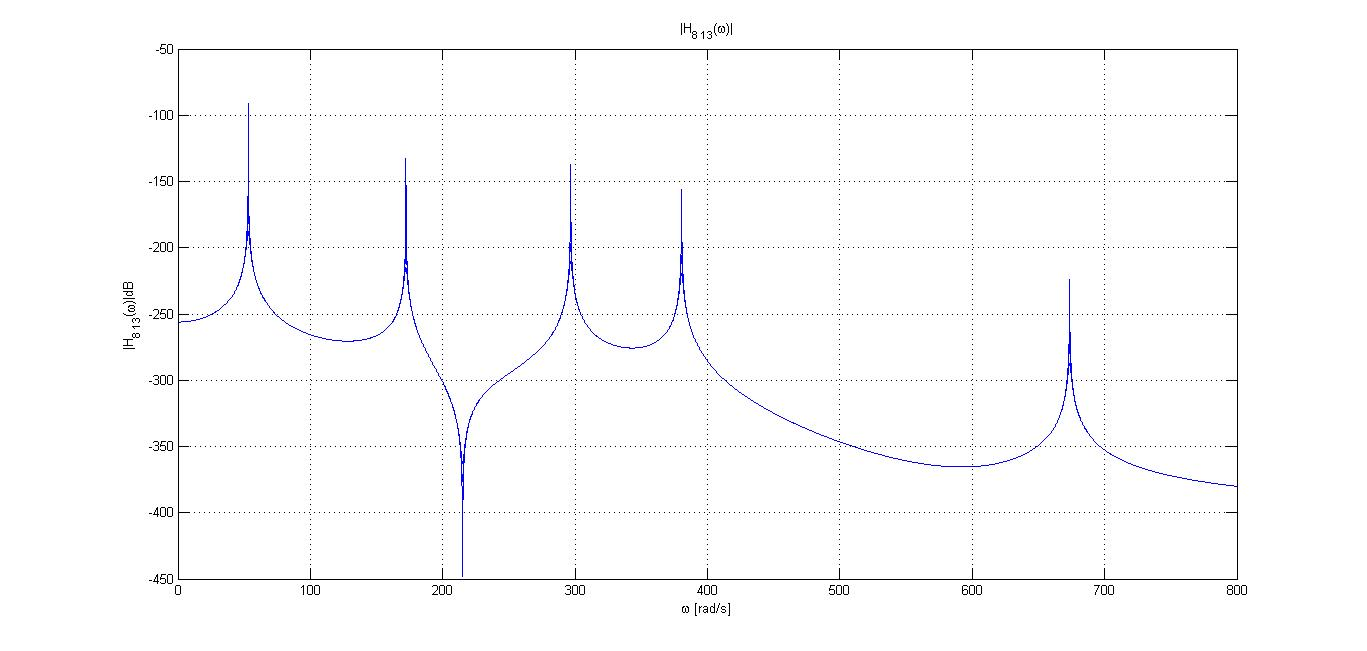
\includegraphics[width=150mm]{Immagini/hijt3}
\caption{Matrice di risposta in frequenza}
\end{figure}\\
Dal grafico si possono osservare diverse cose.\\
Vediamo innanzitutto che in prossimit\'a delle pulsazioni proprie del sistema il modulo di $H_{8,13}(\omega)$ tende a +\(\infty\) (condizione di risonanza), inoltre osserviamo che nonostante abbiamo calcolato $ H_{8,13}(\omega)$ considerando un numero pari a 6 modi di vibrare, il diagramma presenta solo 4 picchi che tendono a +\(\infty\), in particolare non figurano i picchi corrispondenti al modo 3 e al modo 6, questo perch\'e come ci pu\'o vedere dalla figura sotto, che riporta i singoli termini della sommatoria  di $H_{8,13}(\omega)$, i termini corrispondenti al modo 3 e 6 contribuiscono molto poco alla definizione di $H(\omega)$.\\
Un'altra osservazione che si pu\'o fare guardando il grafico,\'e la presenza di un picco che tende a -\(\infty\) tra il secondo picco( corrispondente al secondo modo) e il terzo picco (corrispondente al quarto modo), ricordiamo che il modulo di $H(\omega)$ \'e in dB questo implica che il modulo di $H(\omega)$, tende a 0 in corrispondenza di quella frequenza, questa condizione \'e detta condizione di antirisonanza.\\
\\
\begin{figure}[htbp]
\centering
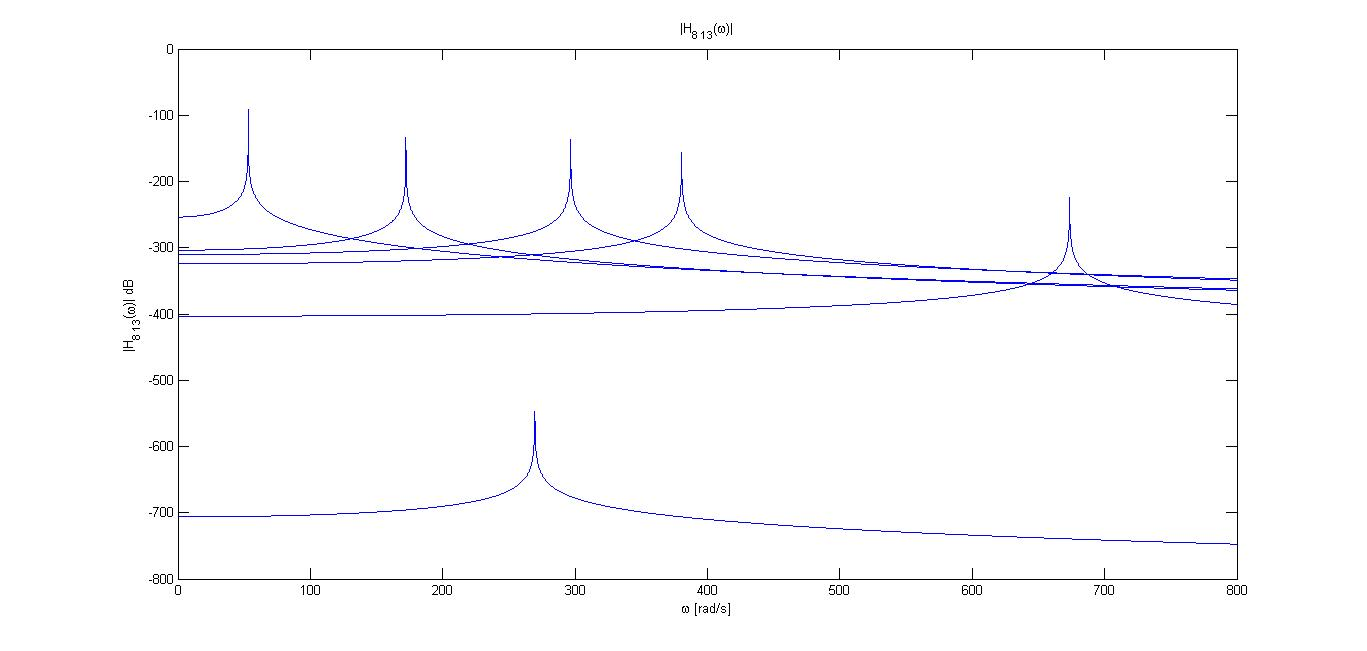
\includegraphics[width=150mm]{Immagini/terminisomma}
\caption{Modulo dei termini sommatoria della matrice di risposta in frequenza in dB}
\end{figure}
\section{Calcolo della matrice delle funzioni di risposta in frequenza in presenza di smorzamento}
In questa sezione abbiamo calcolato la matrice di risposta in frequenza,attraverso l'ausilio di uno script realizzato con MatLab,tra il grado di libert\'a T3 del nodo 8 e il grado di libert\'a T3 del nodo 13, considerando solo i primi 6 modi nella sommatoria dell'espressione modale di $H_{ij}(\omega)$.In particolare riportiamo il valore del modulo $H_{8,13}(\omega)$ in dB,in presenza di smorzamento modale $\zeta$ , in funzione della pulsazione, avendo considerato un unico smorzamento $\zeta$ per tutti e 6  i modi di vibrazione,  il modulo e la fase di $H_{8,13}(\omega)$.Viene inoltre riportato il grafico dei vari termini della sommatoria in funzione della pulsazione.\\
\begin{figure}[htbp]
\centering
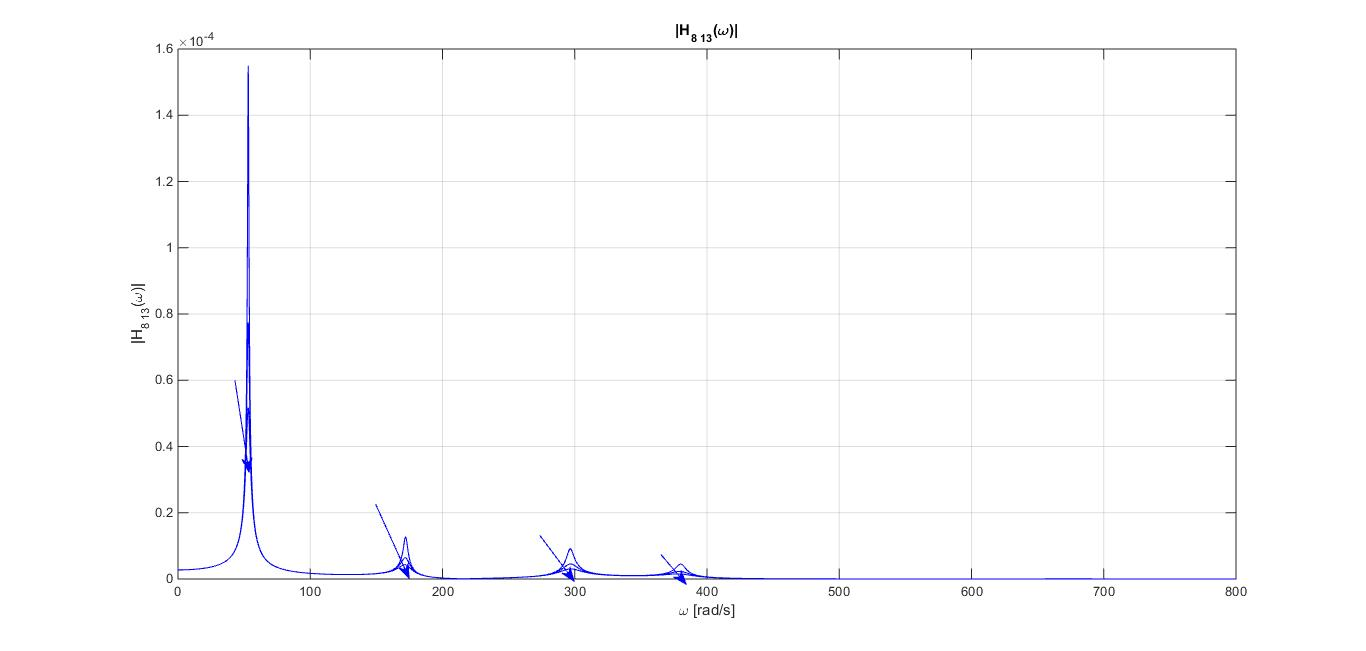
\includegraphics[width=150mm]{Immagini/modulosmorz}
\caption{Modulo matrice di risposta}
\end{figure}\\
\begin{figure}[!h]
\centering
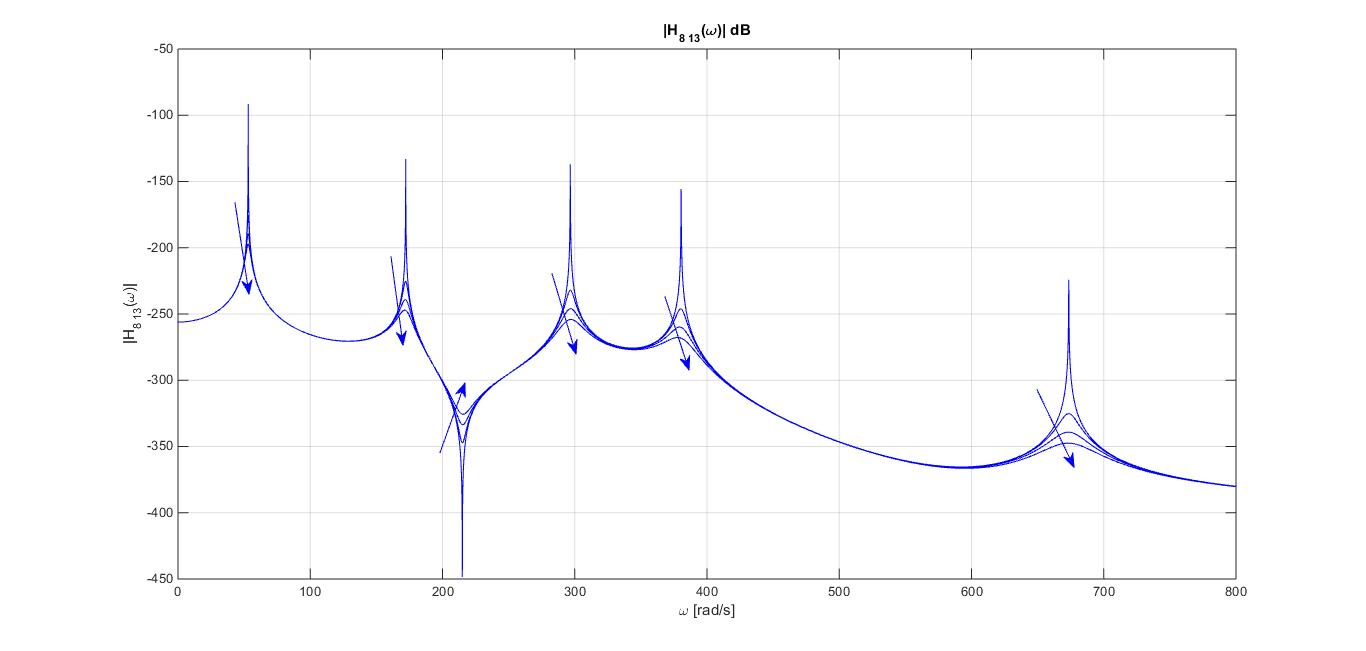
\includegraphics[width=150mm]{Immagini/modulodbsmorz}
\caption{Modulo matrice di risposta in frequenza in dB}
\end{figure}\\
\newpage
Come si puo notare dal grafico i picchi diventano sempre meno pronunciati all'aumentare dello smorzamento, (abbiamo fatto variare lo smorzamento da 0 a 0.03), e pi\'u larghi.
Inoltre si nota che man mano che la pulsazione aumenta,il picco diventa sempre meno pronunciato e pi\'u largo,come ci aspettavamo dalla teoria,questo effetto \'e pi\'u visibile nel grafico riporta nella figura sottostante, dove vengono graficati i termini della sommatoria di H.
Notiano anche come la condizione di antirisonanza,diventa sempre meno accentuata.\\
\begin{figure}[htbp]
\centering
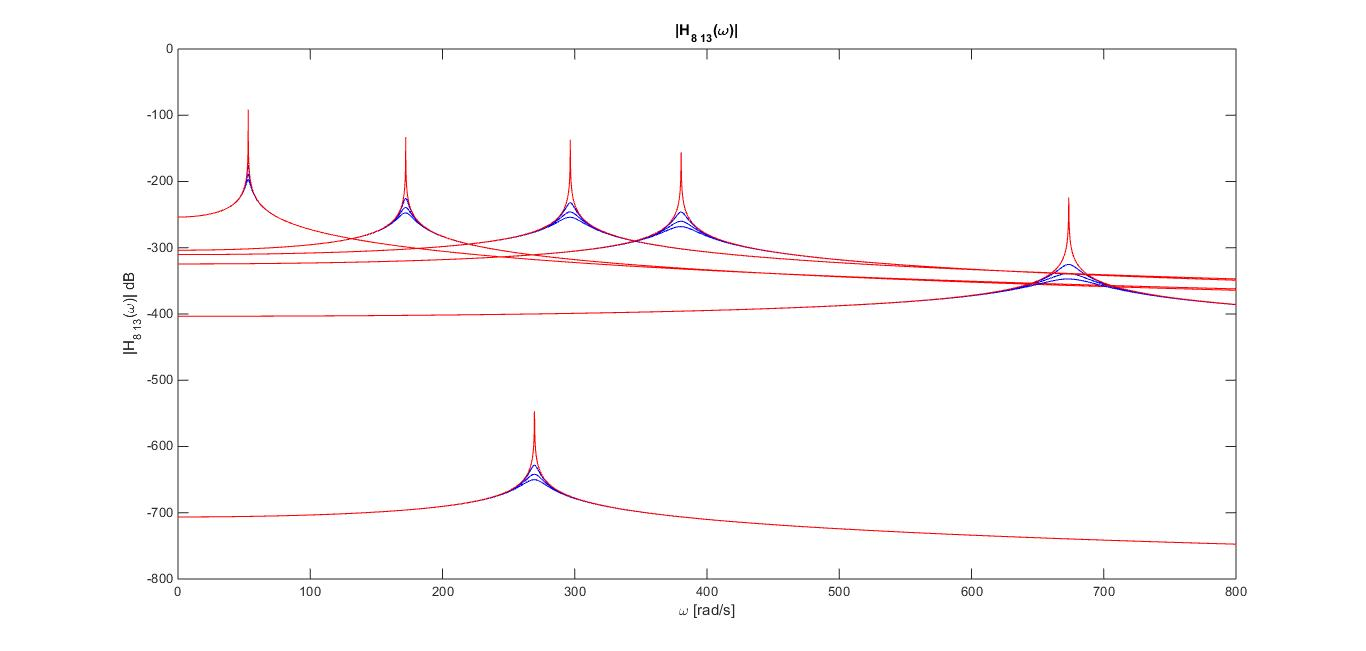
\includegraphics[width=150mm]{Immagini/terminisommasmorz}
\caption{Modulo dei termini sommatoria della matrice di risposta in frequenza in dB}
\end{figure} \\
Infine \'e stata riportata la fase di H, si nota come nel caso di smorzamento nullo l'argomento di H assume valori: 0 +$\pi$ e -$\pi$, questo perch\'e H \'e reale in questo caso.
All'umentare dello smorzamento H diventa immaginario e la sua fase assume tutti i valori compresi tra -$\pi$ e +$\pi$.
Nel caso smorzato la fase di H \'e importante per capire quanto \'e sfasata la risposta del grado di libert\'a T3 del nodo 8 rispetto al carico che agisce sul grado T3 del nodo 13.
\begin{figure}[htbp]
\centering
\includegraphics[width=150mm]{Immagini/Fase}
\caption{Fase}
\end{figure} \\
\newpage
Gli stessi ragionamenti fatti sulla matrice $H_{8,13}$($\omega$) tra il grado di libert\'a T3 di 8 e il grado di libert\'a T3 del nodo 13 possono essere fatti considerando  $H_{8,13}$($\omega$) tra il grado di libert\'a T3 di 8 e il grado di libert\'a T1 del nodo 13.\\
Le stesse considerazioni valgono anche nel caso del termine  $H_{8,13}$($\omega$) tra il grado di libert\'a T1 di 8 e il grado di libert\'a T3 del nodo 13, di cui si riporatno sotto i grafici ottenuti con Matlab.
\newpage
\begin{figure}
\centering
\subfloat[][\emph{Matrice di rispostanza in frequenza}.]
{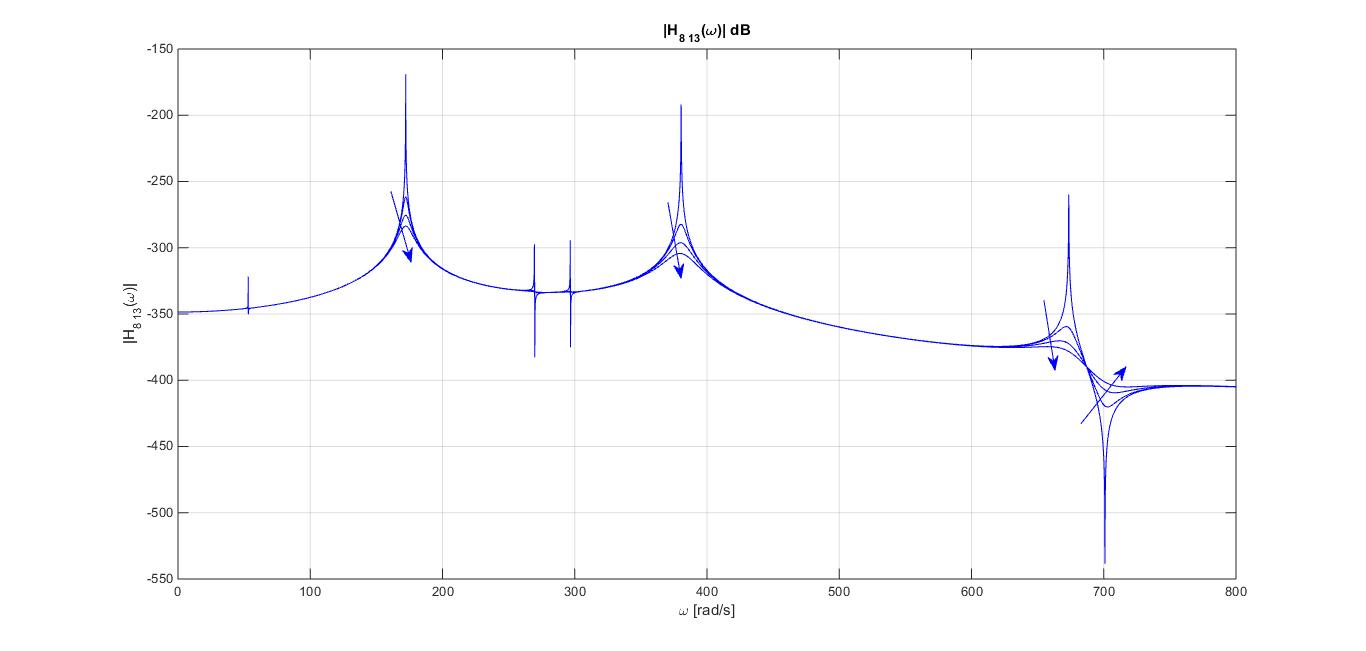
\includegraphics[width=.45\textwidth]{Immagini/matricesommat3t1.jpg}} \quad
\subfloat[][\emph{Modulo dei termini sommatoria della matrice di risposta in frequenza in dB}.]
{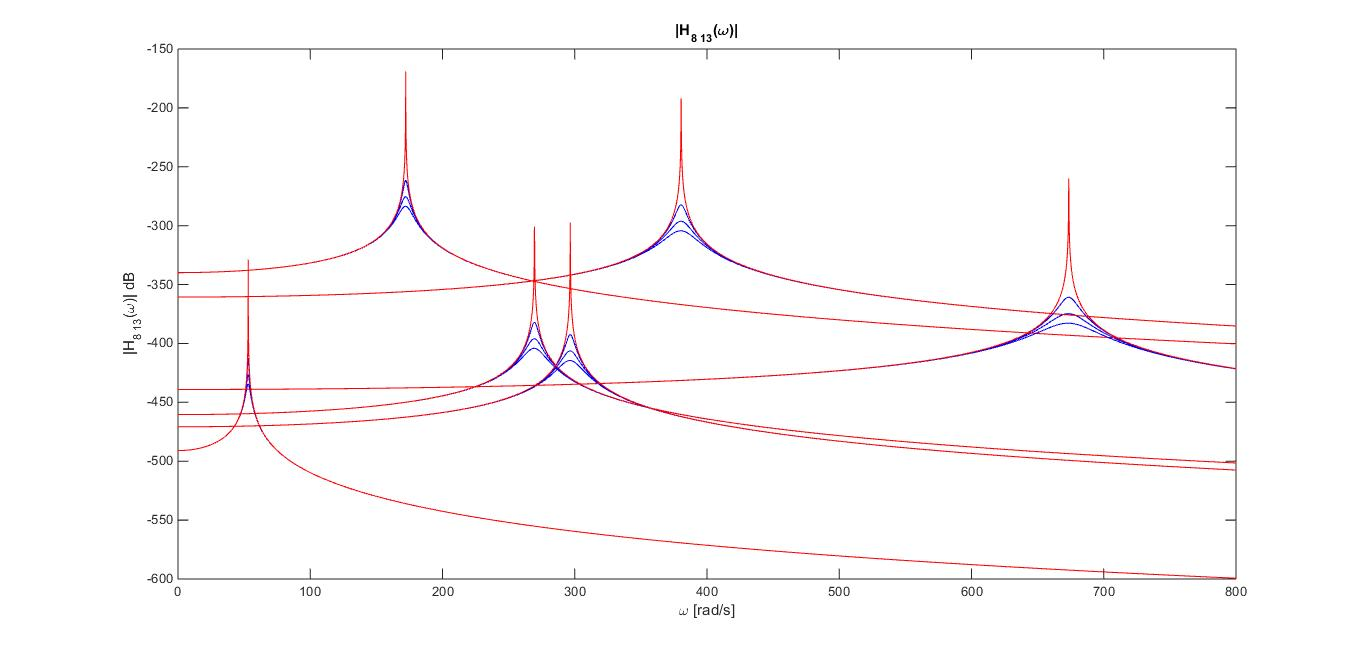
\includegraphics[width=.45\textwidth]{Immagini/terminisommat3t1.jpg}} \\
\subfloat[][\emph{Fase}.]
{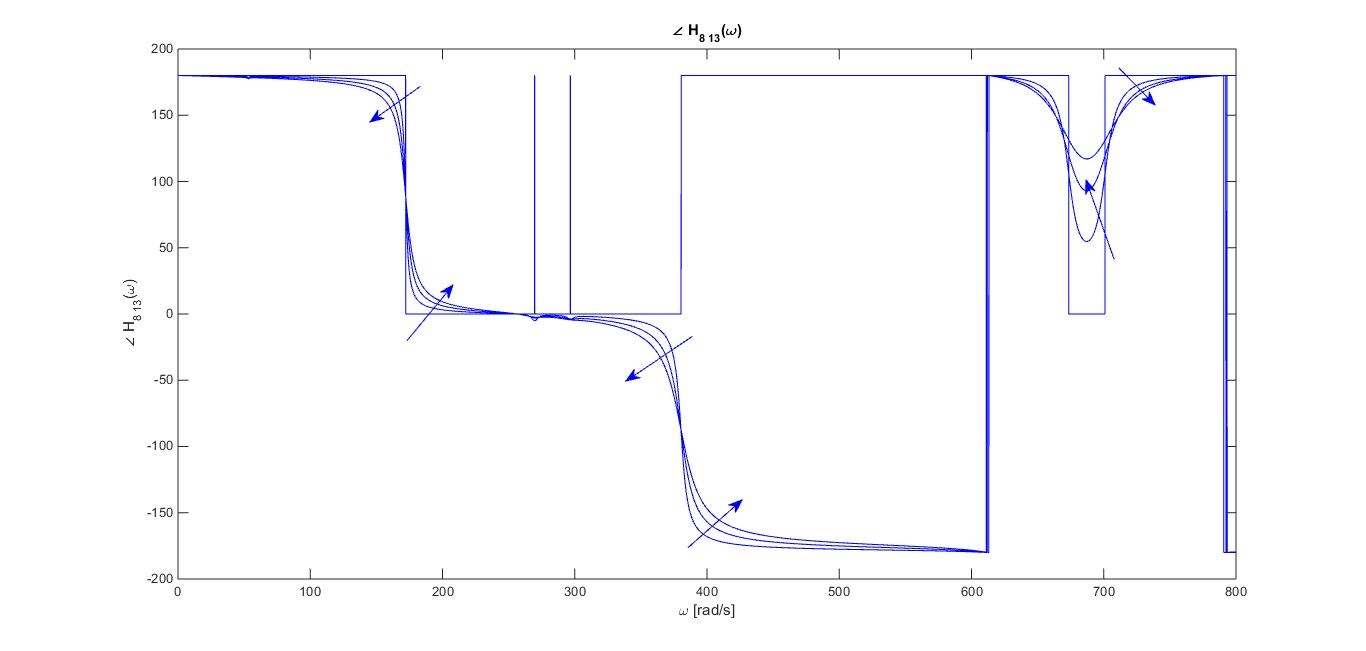
\includegraphics[width=.45\textwidth]{Immagini/faset3t1.jpg}}
\caption{}
\label{fig:subfig}
\end{figure}
\section{Modi flessionali attorno a x caso "appoggio-appoggio"}
In questa sezione si analizzeranno i modi della stessa struttura in una diversa configurazione, in particolare sono state cambiate le condizioni al contorno: togliendo l'incastro e sostituendolo con un appoggio semplice, e mettendo un appoggio semplice anche dalla parte che prima era libera.
Questo \'e stato possibile cambiando i SPC nel bulk data del file "analisi-modale.dat" inibendo i gradi di libert\'a T1 T2 T3 R2 R3 (12356) nei nodi 22,36,28 e 42. Sono stati calcolati i modi di questa configurazione e sono stati individuati i modi flessionali attorno a x, quest'ultimi sono stati confrontati, anche con ausilio di plot grafici realizzati con MatLab, con quelli ottenuti analiticamente dalla teoria della trave di cui si riporta la formula.
\begin{equation}
\omega_{n}=(\frac{n\pi}{l})^2\sqrt{\frac{EI}{\mu}}\qquad \phi(x)=Csin(\frac{n\pi x}{l})\qquad n=1,2,3...
\end{equation}
\begin{center}
\begin{tabular}{cccc}
\hline
\multicolumn{1}{c}{Modo analitico} & Modo FEM &  $\omega_{n }$ Analitica & $\omega$ FEM\\
\hline
  1 &   1 & 122.1647 & 189.4735 \\  
  2 &   4 & 488.6589 & 536.2935 \\  
  3 &   7 & 1099.4825 & 1056.1150 \\  
  4 &   9 & 1954.6355 & 1487.5120 \\  
\hline
\end{tabular}\\
\end{center}
\newpage
\begin{figure}
\centering
\subfloat[][\emph{Modo 1 appoggiato-appoggiato}.]
{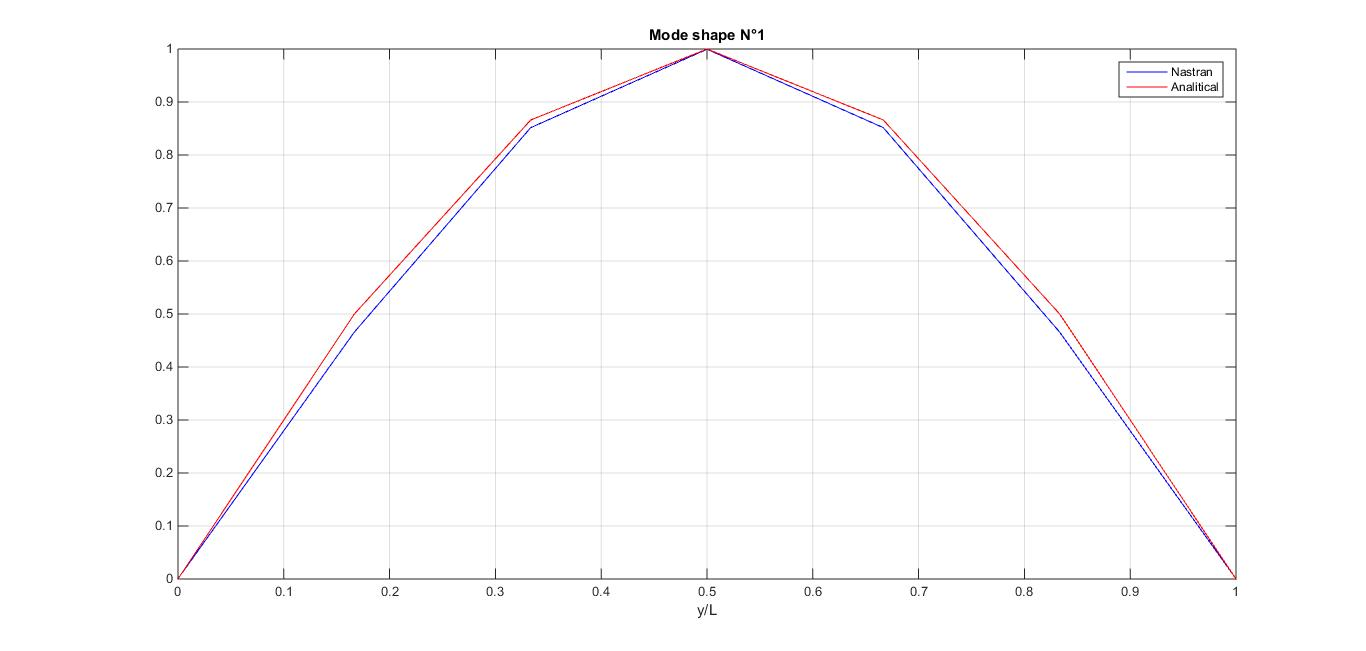
\includegraphics[width=.45\textwidth]{Immagini/modo1app.jpg}} \quad
\subfloat[][\emph{Modo 2  appoggiato-appoggiato}.]
{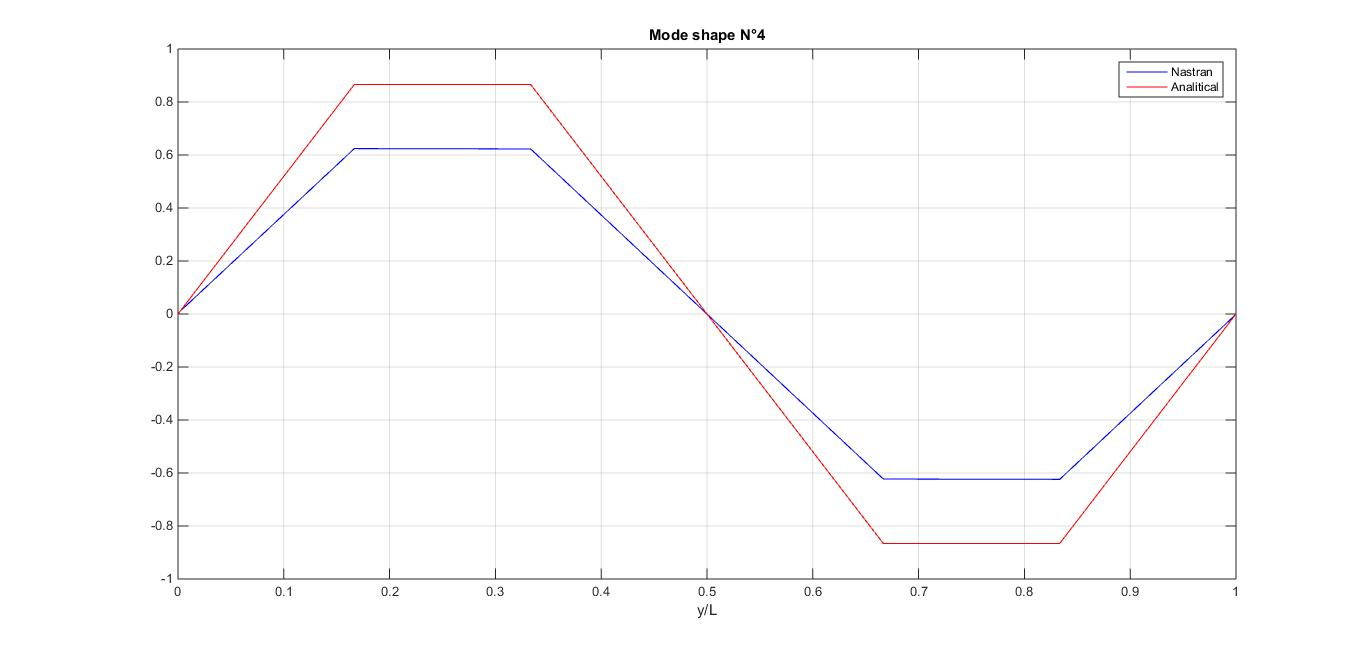
\includegraphics[width=.45\textwidth]{Immagini/modo4app.jpg}} \\
\subfloat[][\emph{Modo 3  appoggiato-appoggiato}.]
{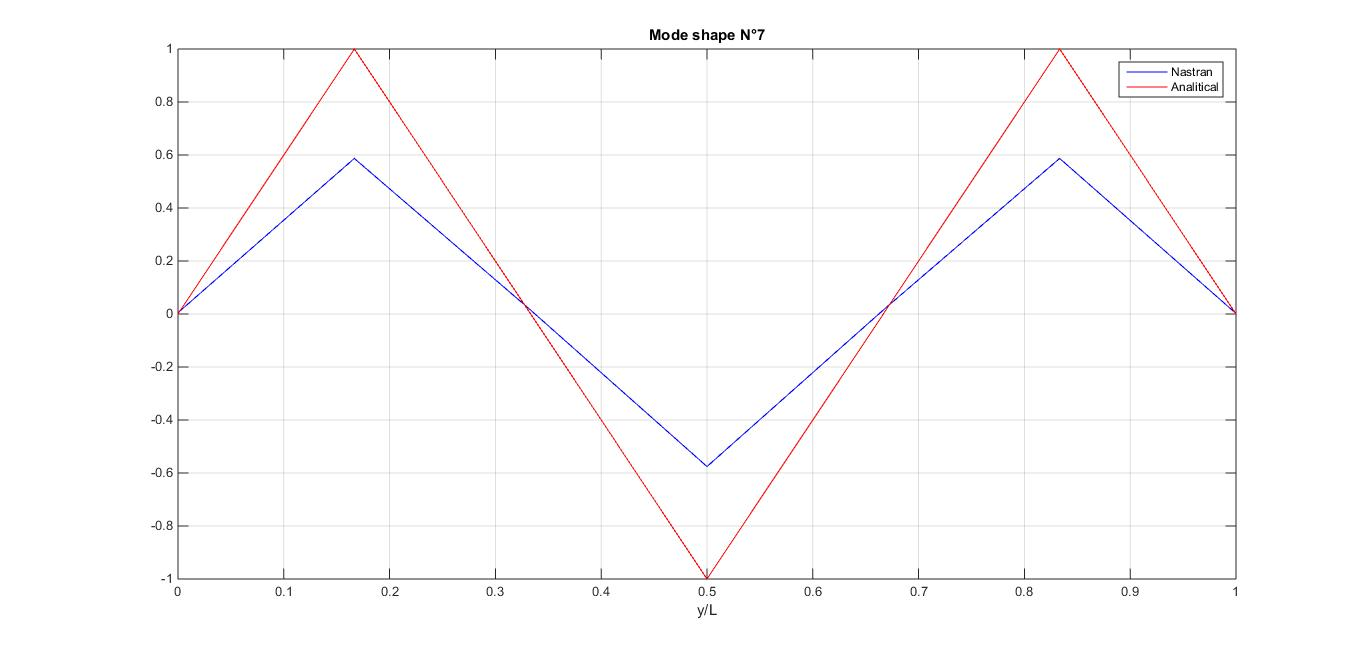
\includegraphics[width=.45\textwidth]{Immagini/modo7app.jpg}} \quad
\subfloat[][\emph{Modo 4  appoggiato-appoggiato}.]
{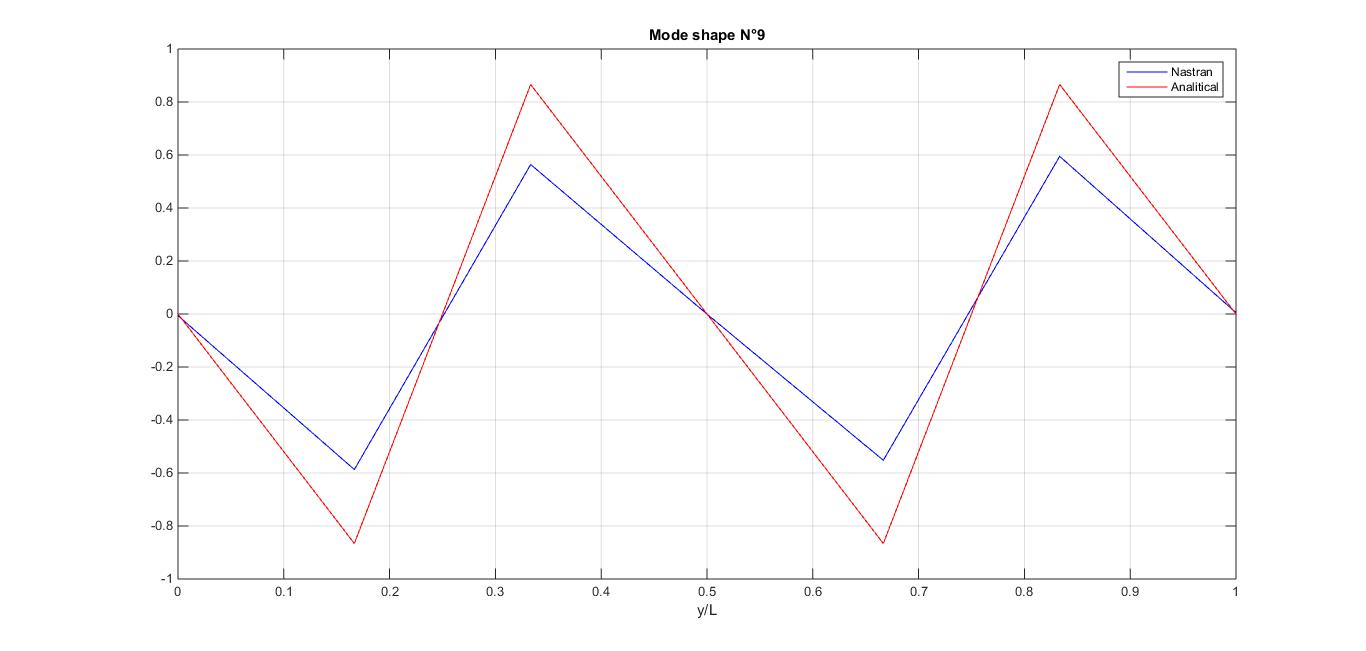
\includegraphics[width=.45\textwidth]{Immagini/modo9app.jpg}}
\caption{}
\label{fig:subfig}
\end{figure}
\end{document}
